\documentclass{beamer}
\usepackage{graphicx}
\usepackage{listings}

\title{Template Metaprogramming}
\subtitle{Or: How I Learned to Stop Worrying and Love the Angle Brackets}
\author{Murray Colpman}

\AtBeginSection[]
{
  \begin{frame}
    \frametitle{Table of Contents}
    \tableofcontents[currentsection]
  \end{frame}
}

\begin{document}
\lstset{language=C++,
                basicstyle=\ttfamily,
                keywordstyle=\color{blue}\ttfamily,
                stringstyle=\color{red}\ttfamily,
                commentstyle=\color{green}\ttfamily,
                morecomment=[l][\color{magenta}]{\#}
}

  \frame{\titlepage}
  \section{Intro}
  \begin{frame}
    \frametitle{WHY?!}
    \begin{itemize}
      \pause
      \item Adds a lot more power to generic programming
        \pause
        \begin{itemize}
          \item Useful for writing libraries, generally used over Java's
            dynamic polymorphism pattern where convenient
          \pause
          \item Implement static polymorphism (Curiously Recurring Template
            Pattern)
        \end{itemize}
      \pause
      \item Run code evaluable at compile time at compile time.
      \pause
      \item Harness the true power of the type checker
      \pause
      \item Terrify and impress people
    \end{itemize}
  \end{frame}
  \begin{frame}
    \frametitle{WHY?! (cont'd)}
    Templates are free at runtime in terms of time complexity, but do add to
    binary size.
    
    \pause

    They might also add to compile time, but is that really a bad thing?

    \pause

    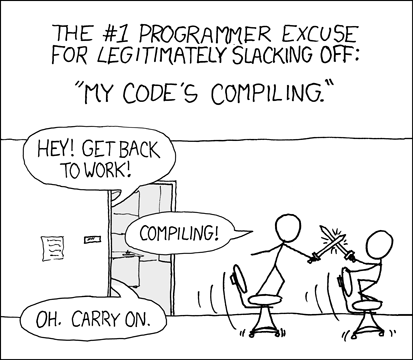
\includegraphics[height=0.5\textheight]{compiling} % magic
  \end{frame}
  \begin{frame}
    \frametitle{Some notes}
    \begin{itemize}
      \pause
      \item Mostly covering C++03
      \pause
      \item Assumes you remember our template lecture
      \pause
      \item I'm not an expert
    \end{itemize}
  \end{frame}
  \section{Template Metaprogramming Theory}
  \begin{frame}[fragile]
    \frametitle{What is TMP?}
    \pause
    It was recognised that people needed to commit atrocities using macros in
    order to get sensible generic programming in the earliest versions of C++.
    \pause

    \begin{lstlisting}
#define TYPE int
#include <insanity.h>
#undef TYPE

#define TYPE double
#include <insanity.h>
#undef TYPE
    \end{lstlisting}

    \begin{itemize}
      \pause
      \item Templates were introduced to make the world a less horrible place.
      \pause
      \item Templates are flexible and Turing-complete.
      \pause
      \item Template metaprogramming is the use of these more advanced features
        of templates to produce code at compile-time.
      \pause
      \item Template metaprogramming is a functional language(!)
    \end{itemize}
\end{frame}
  \begin{frame}
    \frametitle{Mappings to functional languages}
    Using classes or structs:
    \begin{itemize}
        \pause
        \item Integer and type input through template arguments
        \pause
        \item Integer output represented by static const or enum values
        \pause
        \item Type output represented by typedefs
        \pause
        \item Branching uses template specialisation as pattern matching
        \pause
        \item Iteration uses recursion (instantiating new type using same
          template)
    \end{itemize}
  \end{frame}
  \section{Examples}
  \begin{frame}
    \frametitle{Curiously Recurring Template Pattern}
    \pause
    Implementing static polymorphism.
  \end{frame}
  \begin{frame}
    \frametitle{How to terrify interviewers}
    \pause
    ``Proper'' functional programming to generate constants.
  \end{frame}
  \begin{frame}
    \frametitle{Using templated functions to mix in runtime code}
    \pause
    A useful technique.
  \end{frame}
  \begin{frame}
    \frametitle{Static decision making}
    \pause
    An alternative to macros for making decisions dependent on the compile-time
    environment.
  \end{frame}
  \begin{frame}
    \frametitle{Abstract syntax trees}
    \pause
    Implementing a domain-specific language with ASTs.
  \end{frame}
  \section{SFINAE}
  \begin{frame}
    \frametitle{Substitution Failure Is Not An Error}
    \begin{itemize}
      \pause
      \item Templates possibly have very generic names and accept any type
      \pause
      \item C++ needed a way of filtering out templates that had the right
        signature but where where the names referred to simply didn't exist (ie
        false positives)
      \pause
      \item So, when looking for specialisations to use, the C++ compiler drops
        any which would result in an error when substituting the parameters
        (with certain defined limits), without generating an error.
      \pause
      \item How can we abuse this?
    \end{itemize}
  \end{frame}
  \begin{frame}
    \frametitle{Reasoning about types}
    \pause
    You can test for a feature of a type by abusing function overloads.
  \end{frame}
  \begin{frame}
    \frametitle{enable\_if and others}
    \pause
    A common use is an "enable\_if" macro. It's a very simple macro but one
    that can be used to conditionally enable other templates.
  \end{frame}
  \section{C++11 Improvements}
  \begin{frame}
    \frametitle{decltype}
    \pause
    decltype allows you to get the declared type of any expression.

    \pause

    It's very useful for TMP, used a lot in the standard library.

    \pause

    For example, makes it much easier to do SFINAE reasoning about methods.
  \end{frame}
  \begin{frame}
    \frametitle{Variadic templates}
    \pause
    You can now have arbitrary lists of arguments in templates, and handle them
    in a really nice manner.

    \pause

    You can use it to produce arbitrary-length tuples, for instance, among many
    many other things.
  \end{frame}
  \begin{frame}
    \frametitle{constexpr}
    \pause
    Lets you declare variables and functions as ``constexpr'' to tag that they
    can be evaluated at compile-time.
    
    \pause
    
    Can be used to replace the Fibonacci example above with something much
    neater, eliminating TMP altogether, but can also be used in conjunction with
    TMP to do things in a much neater way.

    \pause

    Also useful is static\_assert for compile-time errors.
  \end{frame}
  \begin{frame}
    \frametitle{Template aliases}
    \pause
    Let you alias templates (without instantiating them) in the same way that
    you can have typedefs.
    
    \pause

    Uses the ``using'' keyword.
  \end{frame}
  \begin{frame}
    \frametitle{Type traits}
    \pause
    Allow you to reason about types using simple interface at compile-time. Can
    be used in conjunction with TMP or with constexpr functions.
  \end{frame}

\end{document}
